\documentclass[a4paper,11pt]{article}
\usepackage{amsthm}
\usepackage{amsmath}
\usepackage{amssymb}
\usepackage{color}
\usepackage{graphicx}
\usepackage{fullpage}
\usepackage[]{units}
\usepackage{hyperref}
\usepackage{verbatim}
\usepackage{tikz}
\usepackage[ruled]{algorithm2e}
\usepackage{fontenc}
\usepackage[utf8]{inputenc}
\usepackage{mathtools}
\usetikzlibrary{arrows}
\newtheorem{theorem}{Theorem}
\newtheorem{lemma}{Lemma}[section]
\newtheorem*{remark}{Remark}
\newtheorem{proposition}[theorem]{Proposition}
\renewcommand{\thefootnote}{\fnsymbol{footnote}}
\newcommand{\norm}[1]{\lVert#1\rVert}
       % define the title
       \author{Nikhil J. Nathwani}
       \title{Playoff Success Orbit}
       \begin{document}
       % generates the title
       \maketitle

\section{Goal}
	The goal is to get a sense for how well a team will perform in the playoffs based on the success of similar playoff teams of the past. The method used to compare teams should not be significantly influenced changes in rules (e.g. the advent of the 3-point line) or trends (e.g. the recent affinity for small-ball) over the years.

\section{kNN Algorithm}
	The k-Nearest Neighbors (kNN) algorithm is tailor-made for making predictions based on prior information.

\subsection{How it works}
If you're already familiar with kNN, you don't need to read this subsection.

The basis of kNN is: given an unclassified object, look into your training data for the $k$ most similar objects, and take a majority vote amongst those to determine a classification for the object in question. The terms \emph{training data} and \emph{most similar} ought to be defined -- they can be explained by example:

Suppose you pick up a flower and would like to identify what type of flower it is. So you take measurements: stem length, petal width, etc. These measurements together form a vector of \emph{attributes} for the flower. Also at your disposal is a trove of pre-collected flower data of the form (attribute vector, type of flower). Note that the flowers in this data trove -- the \emph{training data} -- are already classified, i.e. their type is known.

What can we do to guess precisely what type of flower is in your hand? You can look at the flowers within our training data whose attribute vectors closely match that which we measured, and classify your flower based on the labelings of those most similar flowers. The notion of \emph{most similar} can vary from situation to situation; in this case, it makes sense to use \href{http://en.wikipedia.org/wiki/Euclidean_distance}{Euclidean distance} as our measure, so that the smaller the Euclidean distance between two flowers, the more similar they are. This distance is the \emph{similarity score}.

After calculating the similarity scores for all flowers in our training data, you can look at the $k$ flowers with the best similarity scores ($k$ can be chosen arbitrarily, or a ``smart'' $k$-value can be experimentally determined via cross-validation, which is outside the scope of this discussion). kNN looks at the types (a.k.a. \emph{labels}) of these $k$ most similar flowers and picks the mode. So, if k=10 and the types of the most similar flowers include 7 sunflowers, 2 irises, and 1 rose, we would label the flower in your hand as a sunflower.

\subsection{Application to Basketball}
\begin{itemize}
\item The \emph{attribute vectors} are the team-level stats available on basketball-reference.com for each team (see ``List of Stats in Attribute Vector'' section of Appendix for a complete list). The Data Preprocessing section has more information on the kind of data used. 

\item The \emph{training data} is comprised of the attribute vectors of past playoff teams, which are \emph{labelled} by the number of playoff series won by those teams.
	
\item The \emph{similarity score} is the inverse Euclidean distance\footnote{It's the inverse of Euclidean distance because the small the distance between two attribute vectors, the more similar } between attribute vectors once those vectors are properly scaled (the Data Processing section explains how this scaling is done).
\end{itemize}

To predict the number of playoff wins for team $X$, a weighted average of playoff series wins is taken amongst the $k$-nearest neighbors of $X$, using the similarity scores as weight. I call this average the \emph{weighted win score} (WWS). For example, if $k=3$ and the nearest neighbors of team $X$ are:

\begin{center}
    \begin{tabular}{| c | c | c |}
    \hline
    Team & Distance & Series Wins \\ \hline
    $A$ & 2 & 3  \\ \hline
    $B$ & 0.5 & 0 \\ \hline
    $C$ & 1.5 & 1  \\
    \hline
    \end{tabular}
\end{center}

Then the WWS of team $X$ is:

\begin{center}
$\frac{(\nicefrac{1}{2})(3) + (\nicefrac{1}{0.5})(0) + (\nicefrac{1}{1.5})(1)}{(\nicefrac{1}{2})+(\nicefrac{1}{0.5})+(\nicefrac{1}{1.5})} = \frac{13}{19}$
\end{center}

Upon calculating the WWS for all 16 playoff teams of 2014, I simulate each playoff matchup by deeming the winner to be the team with the larger WWS. The ``WWS Rankings \& Playoff Simulation'' section of the Appendix shows the results of this simulation, and a table ranking the 2014 playoff teams by WWS.

\section{Data Preprocessing}
The following are transformations made to the historical data, along with the advantages and drawbacks associated with them.

\begin{enumerate}

\item Only teams that played from the '79-'80 season onwards are considered, because this is the year that that three-point line was created.
\begin{itemize}
\item \textbf{Advantages:} Three-point field goals have changed the style of basketball being played, so it makes sense to only judge today's teams against those that also were also affected by the three-point arc. Moreover, excluding pre-1979 teams avoids the issue of having empty entries in our attribute vectors (i.e. the entries relating to three-pointer statistics).
\item \textbf{Drawbacks:} Excluding seasons reduces the size of our training data, which can lead to \textcolor{blue}{\underline{\href{http://en.wikipedia.org/wiki/Overfitting}{overfitting}}} when performing kNN.
\end{itemize}

\item Only regular season ranks are used as entries in the attribute vectors, e.g. a team's assist rank amongst the entire league is used in its attribute vector, not the total number of assists the team accumulated throughout the regular season.
\begin{itemize}
\item \textbf{Advantages:} Attribute vectors are robust against the ebbs and flows of overall league play across seasons\footnote{E.g. in seasons where defensive performance spikes league-wide and scoring totals decrease, the team leading in overall points may have a much lower point total than teams in 2014. But that team's playoff success is based on their \emph{relative} performance against their peers, so the point total shouldn't matter as much as the fact that they led the league on that front.}.
\item \textbf{Drawbacks:} Regular season league ranks include non-playoff teams, so some team totals may be notably impacted by poor competition. Also, matchups aren't taken into account, so although a team may be ranked first in total points, their point total in individual games would likely drop when facing a top defensive team in the playoffs. 
\end{itemize}

\item Each entry of the attribute vector is \textcolor{blue}{\underline{\href{http://en.wikipedia.org/wiki/Feature_scaling\#Methods}{rescaled}}} to a [0,1] range. 
\begin{itemize}
\item \textbf{Advantages:} Expansion teams lead to differing numbers of teams across seasons. So, league ranks go from 1 to 22 in some years, while today they go from 1 to 30. This makes an impact when calculating Euclidean distance, but by rescaling, this impact is more uniform, instead of being skewed toward the left end of the range. 
\item \textbf{Drawbacks:} It may be the case that some team stats are more important than others when predicting playoff success, and thus deserve more weight, but this isn't the case since all stats are rescaled in the same manner\footnote{There are machine learning techniques for \textcolor{blue}{\underline{\href{http://en.wikipedia.org/wiki/Feature_selection}{feature selection}}} that can be used to determine smarter scaling procedures for each attribute -- this may be revisited in future iterations of the data visualization.}.
\end{itemize}
 
\end{enumerate}


\section{Appendix}
\subsection{List of Stats in Attribute Vector}
	All of the following stats are included in the attribute vector of each team. Below they are ordered in the same way in which they're presented in basketball-reference.com\footnote{For example, \textcolor{blue}{\underline{\href{http://www.basketball-reference.com/teams/BOS/2014.html\#all_team_stats}{here}}}.}. It's important to note that only regular season league ranks are used in each vector, e.g. a team's assist rank amongst the entire league is used in its attribute vector, not the total number of assists the team accumulated throughout the regular season.												

\subsubsection{Team Key Stats}
FG, FGA, FG\%, 3P, 3PA, 3P\%, 2P, 2PA, 2P\%, FT, FTA, FT\%, ORB, DRB, TRB, AST, STL, BLK, TOV, PF, PTS

\subsubsection{Opponent Key Stats}
FG, FGA, FG\%, 3P, 3PA, 3P\%, 2P, 2PA, 2P\%, FT, FTA, FT\%, ORB, DRB, TRB, AST, STL, BLK, TOV, PF, PTS

\subsubsection{Team Miscellaneous Stats}
MOV, SOS, SRS, ORtg, DRtg, Pace, FTr, 3PAr

\noindent \textbf{Offensive Four Factors:} eFG\%, TOV\%, ORB\%, FT/FGA

\noindent \textbf{Defensive Four Factors:} eFG\%, TOV\%, DRB\%, FT/FGA


\subsection{WWS Rankings \& Playoff Simulation}

\subsubsection{WWS Rankings}
\begin{table}[ht]
\centering
    \begin{tabular}{ccc}
    Rank & Team & WWS               \\
    1    & SAS  & 1.823596857911819 \\
    2    & OKC  & 1.766564183089487 \\
    3    & POR  & 1.601486869472524 \\
    4    & LAC  & 1.343669734428170 \\
    5    & HOU  & 1.320601629355732 \\
    6    & GSW  & 1.304062499300451 \\
    7    & MIA  & 1.298095116510139 \\
    8    & IND  & 1.173332130373204 \\
    9    & CHI  & 1.034751760110605 \\
    10    & TOR  & 0.79427781584533 \\
    11    & DAL  & 0.74654336865026 \\
    12    & MEM  & 0.62126865595580 \\
    13    & BRK  & 0.60635275834279 \\
    14    & CHA & 0.55906949219646 \\
    15    & ATL  & 0.54013724954760 \\
    16    & WAS  & 0.50992579841762 \\
    \end{tabular}
\end{table}

\subsubsection{Playoff Simulation}
Correct predictions written in green, incorrect predictions in red. As can be seen on the next page, 13 of 15 predictions led to correct outcomes. 

\begin{center}
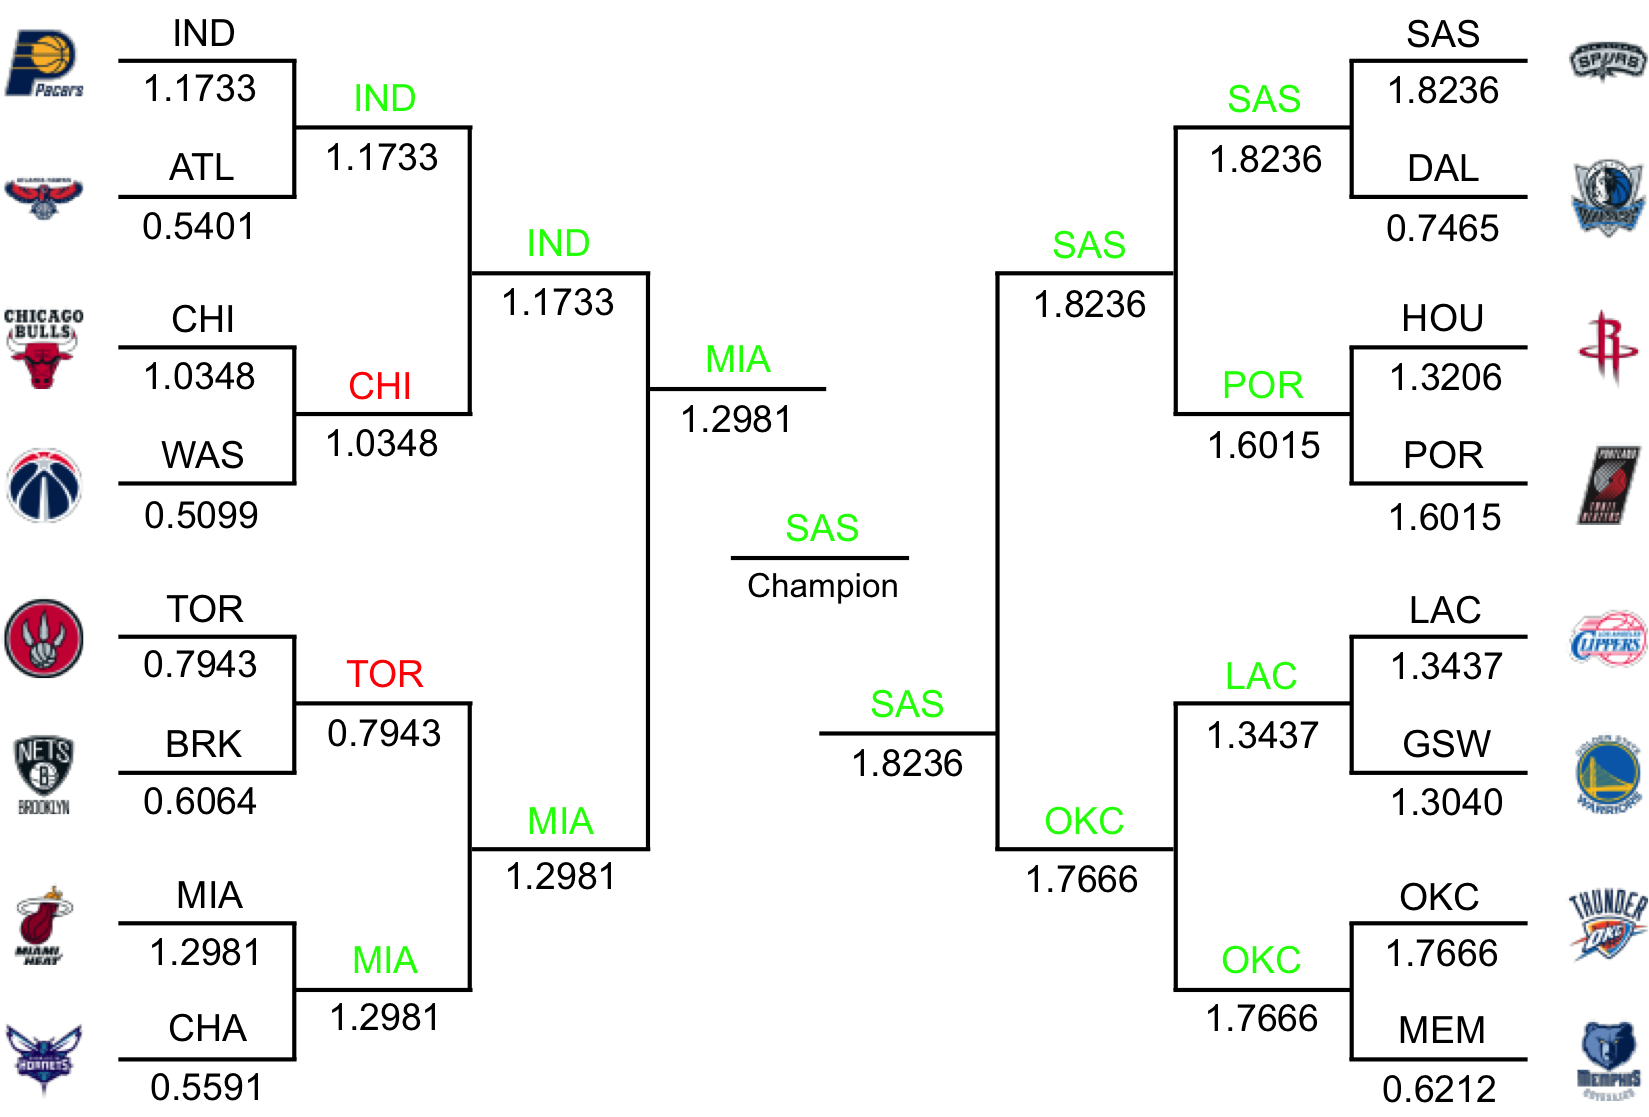
\includegraphics[scale=0.6]{bracket}
\end{center}


\end{document}